\section{Results and discussion}\label{sec:results}

In this section, we detail the findings of our study. We present the results of the first study in Section~\ref{sec:testGeneration}. It could estimate the performance of the test generation tools for mining Android  Sandboxes, in terms of malware detection. Section \ref{sec:path} present the result of Paths analysis, and Section~\ref{sec:manifest} Manifest file analysis. Section~\ref{sec:implications} cross some results, and present some implications.

\subsection{Effectiveness of Test generation tools on Detecting Malicious apps}\label{sec:testGeneration}

Given a pair of apps, we first perform an exploratory phase at both app versions at a specific test generation tool, for three minutes, as detailed before. After execution, DroidXP produces a dataset with the sensitive APIs that both app versions call. We consider that a test generation tool could construct a sandbox able to detect or do not a specific malware, by comparing the calls to sensitive APIs made by the benign and malign versions of the apps. DroidXP checks if the malicious app version calls other sensitive APIs but is not called by your benign version. If this happens, we consider that the test generation tool under analysis could detect the specific malware.

In the final process, we generate a report that includes a set of observations like the tool name, the number of the repetition (in the range [1..3]), and a boolean value indicating whether or not the malware has been identified. Figure~\ref{fig:accuracy} presents the result of each individual test generation tool in detecting malware at our data set (824 app pair).

Among the malware detected by all test tools, we also check its similarity score. We choose does not to discard any malware based on a selected threshold, since this could affect both false positives and false negatives. For example, if we use a high similarity score for select malware, we will have a low false positive and high false negative. Otherwise, a low similarity score brings high false positives and low false negatives. Zhou et al.\cite{DBLP:conf/codaspy/ZhouZJN12} mention the threshold of 70\% as a good balance to infer whether an app is repackaged or not. Hence, our results also present how many detected malware are above and below this threshold (70\%), at each test tool.\newline
\newline
\textbf{Droidbot:} When using Droidbot to build sandbox, our results present that it could detect a total of $677$ malware among $824$ app pairs in the dataset (82.16\%). Among tools used in our study, Droidbot was the most efficient in terms of the detection of apps with malicious behavior. At other works~\cite{DBLP:conf/wcre/BaoLL18}\cite{DBLP:journals/jss/CostaMMSSBNR22}, Droidbot has been shown to be the most efficient tool, whose resulting sandbox detected the largest number of malicious apps. Among all malicious apps detected, $347$ have a similarity score below 70\% and $330$ above.\newline
\newline
\textbf{Monkey:} The tool part of the Android SDK produced a sandbox that detected $527$ malware out of the dataset (63.95\%). It created the second best efficient sandbox in our study, although it implements the most basic random strategy test~\cite{DBLP:conf/icst/WetzlmaierRP16}\cite{DBLP:conf/kbse/ChoudharyGO15}. $288$ malware detected has similarity score below 70\% and $239$ above.   \newline
\newline
\textbf{Droidmate2:} Droidmate was designed with an explicit goal of monitored calls to Android sensitive methods based on a set of sensitive APIs defined in the framework AppGuard~\cite{DBLP:conf/esorics/BackesGHMS13}. Although it has this specific goal, it sandbox detected $414$ malicious apps (50.24\%). Only a little more than half of the dataset. Among malware detected, $224$ have a score below 70\% and $190$ above.\newline
\newline
\textbf{Humanoid:}  The tool that emulates realistic users had the worst performance in comparison to others, that rely on random testing (such as Monkey). Since Humanoid create human-like test inputs, based on a learned model, we believe that in a simulated environment, its method to generate test inputs is impaired. The resulting sandbox identified 401 malicious apps in our dataset (48.66\%), less than half of the dataset. Regarding similarity score, in view of threshold (70\%), it was the only tool that have less malware with a score below 70\% among all detected, $197$ malware, and more above 70\%, $204$ malware.

\begin{figure}[ht]
\centering
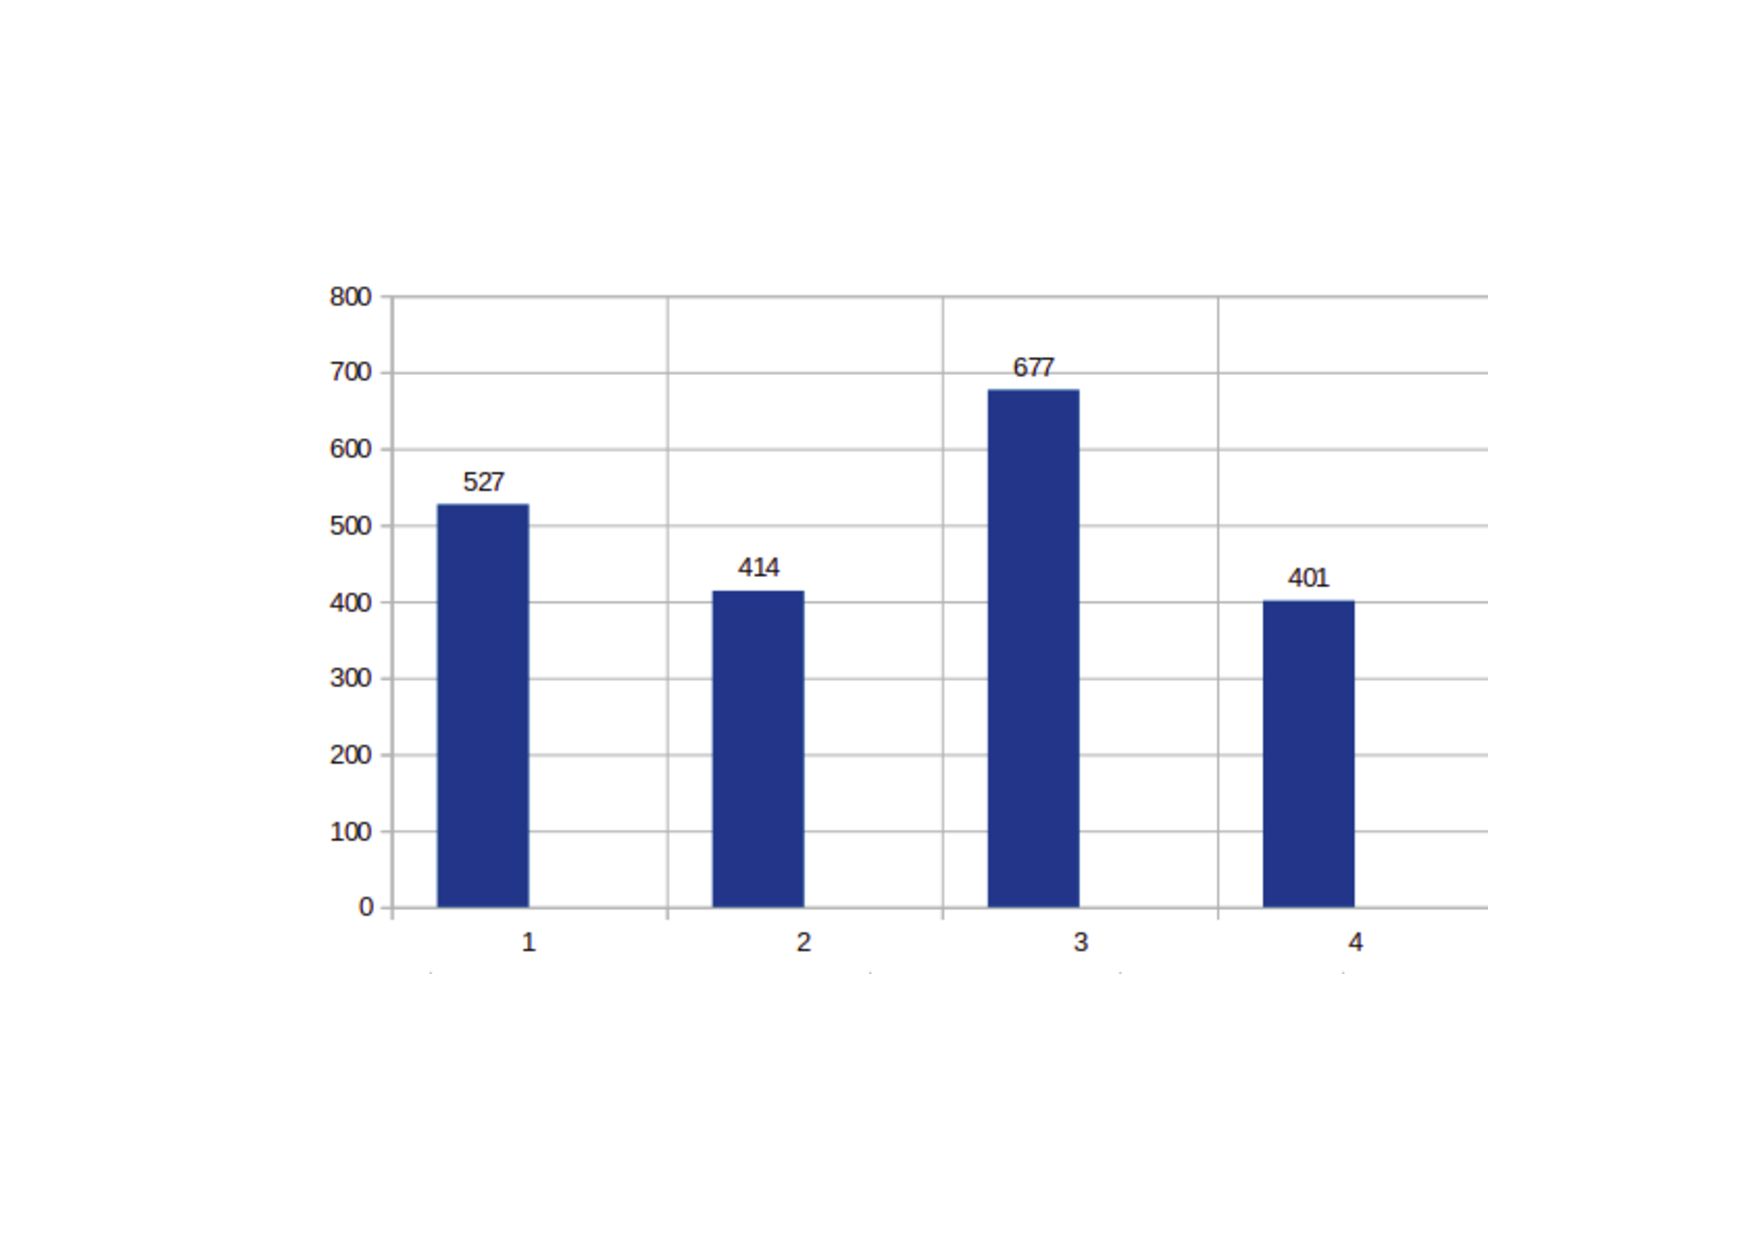
\includegraphics[scale=0.3]{images/accuracy.pdf}
\caption{Accuracy of each test generator tool on malware detection.}
 \label{fig:accuracy}
\end{figure}

\subsection{Path Analysis}\label{sec:path}

Our investigation into malicious apps was also carried out through a Paths analysis. The analysis is conducted checking the callgraph created by Logcat when performance the app pairs, on each test generator. First, we make a filter to collect just the paths between the app entry point and the call to any method sensitive, based on a methods sensitive list from framework AppGuard.

Finally, with both callgraph, from benign and malicious app versions, we compare them. If we spotting differences between any paths, means that the sensitive methods are accessing in a different way from app pairs, and we can consider it as malware.

Because all app pairs detected at our first study, using Mine Sandbox, have naturally different paths, we choose to investigate only app pairs that were not detected at Mine Sandbox approach. Our results show that it is possible to improve malware detection if we also consider the path between app entry point and sensitive methods call.

Table~\ref{tab:pa} summarizes the results of this investigation. The column Execution (NID) shows the number of malware not identified when executing each tool, at mine Sandbox approach. Column  Path Different (PD) shows the number of app pairs, among no identified at first columns, have different paths from the entry point to the sensitive method call. Improve column shows(in percentage) how many the path analysis could improve malware detection if this approach is also considered. We calculate the improvement using Eq.~\eqref{improve}


\begin{table}[ht]
  \caption{Summary of the results of path analysis. }
  \centering
  \begin{small}
 \begin{tabular}{lrrr}
   \toprule
   Tool & Execution (NID) & Path Analysis (PD) & Improve (\%) \\   \midrule
   Monkey &  297 & 157 & 52.86 \\ 
   Droidmate &  410 & 259 & 63.17 \\ 
   Droidbot &  147 & 103 & 70.06 \\ 
   Humanoid &  423 & 27 & 39.71 \\ 
 \bottomrule
 \end{tabular}
 \end{small}
 \label{tab:pa}
\end{table}

\begin{eqnarray}
Improve & = & \frac{Path Analysis (DP) \times 100}{Execution (ND)} 
\label{improve}
\end{eqnarray}

As we can see in Table~\ref{tab:pa}, although Droidbot already had the best accuracy at first study, if we also consider compare paths, Droidbot could benefit the most from working together with this approach. On the other hand, Humanoid that does not identify 423 app pair, the worst performance at first study, do not have good support of the compare path proposal, like other tools, having the accuracy improving at just 39.71\%.

\subsection{Manifest File Analysis}\label{sec:manifest}

We also check some particulars from Manifest file, that point to a likely suspicious behavior, and also could give support to mine Sandobox approach. In section \ref{sec:manifestAnalysis}, we show that an automatic hacking script could inject duplicated permission and actions at Manifest file. We investigated if this happened at pair no detected at first study. We also check if among these pairs, there were requests to new permissions, that were not initially requested by benign version, or if there was an excessive request from permissions at malicious version. Table~\ref{tab:mfa} gives some features of Manifest file from malware not detected at first study. 

\begin{table}[ht]
  \caption{Manifest File with duplicate code.}
  \centering
  \begin{small}
 \begin{tabular}{lccccc}
   \toprule
   Tool & (NID) & (DP) & (DA) & (DP or DA) & (DP and DA) \\   \midrule
   Monkey &  297 & 36 & 44 & 62 & 18 \\ 
   Droidmate &  410 & 48 & 63 & 91 & 20 \\ 
   Droidbot &  147 & 18 & 25 & 36 & 7 \\ 
   Humanoid &  423 & 51 & 61 & 91 & 21 \\ 
 \bottomrule
 \end{tabular}
 \end{small}
 \label{tab:mfa}
\end{table}

Column (NID) indicates the number of malware not detected at first study. It is the same numbers that have been reported at table~\ref{tab:pa} (Execution NID). The second column (DP) indicates how many Manifest files had duplicated permission, among malware at first column (NID). Column (DA) follows the same idea as the previous column, presenting now the duplicated actions. The last two columns present the combination of columns (DP and DA) by logic operators (And/Or).

We deduce that if we have on the same Manifest file, duplicate request permissions, and actions, it was not injected by mistake, and it is a clue that the Manifest file was modified for malicious purposes. Considering this view, $18$ among app pairs do not detect by Monkey tool, had this feature, confirming that they were indeed malware. The same feature we find at $20$ app pair, that was not detected by sandbox build by Droidmate test tool, $7$ and $21$ app pairs by Droidbot and Humanoid respectively. Hence, Humanoid tool had more app pairs with Manifest files with a strong suspicion of malicious modify, among app pairs do not detected by its sandbox. 

Interestingly, among all app pairs at last columns (69 app pairs), just $4$ have the similarity score above 70\%, $2$ from Monkey, $1$ from Droidmate, and $1$ from Humanoid. Other app pairs with very suspicious Manifest file, have a high similarity score, which indeed makes it difficult detection with mine Sandbox approach.

At final analysis, we investigate how many app pairs request more permission than your benign version, featuring a suspicious amount of permission requests. Some works present that a benign Android app normally requests on average $4$ permission, while a malicious apps version requests a median number of $7$ permission\cite{DBLP:conf/soups/FeltHEHCW12}\cite{DBLP:journals/tifs/0029LBKTLC17}. Hence, and our study we investigate how many app pairs have at least $3$ more permission than its benign version. Table~\ref{tab:mp} presents the results.

\begin{table}[ht]
  \caption{Manifest File with more permissions.}
  \centering
  \begin{small}
 \begin{tabular}{lccc}
   \toprule
   Tool & (MP) & (DP) & (NDP) \\   \midrule
   Monkey &  10 & 8 & 2 \\ 
   Droidmate &  11 & 8 & 3 \\ 
   Droidbot &  3 & 1 & 2 \\ 
   Humanoid &  15 & 11 & 4 \\ 
 \bottomrule
 \end{tabular}
 \end{small}
 \label{tab:mp}
\end{table}

The second column (MP) present how many app pairs, no detected by each test tool, have other suspicious feature of Manifest file. It has request at least $4$ or more permission than its benign version. Third and fourth columns (DP)(NDP) presents how many app pair from second columns have duplicated permission or not respectively. As we can see, most of app pair that have excessive permission request, also have duplicated permission in your code. From table~\ref{tab:mp}, we note that test tool Humanoid, has the most apps no detected by mine Sandbox approach with excessive request permission.


\subsection{Implications}\label{sec:implications}